\subsection{Краткое описание}

\begin{frame}
\frametitle{Краткое описание}
  \begin{columns}[T]

    \begin{column}{.4\textwidth}
     \begin{block}{Краткое описание}
        Петрозаводский государственный университет – крупнейший многопрофильный классический вуз Европейского Севера России.
    \end{block}
    \end{column}

    \uncover<2>{
    \begin{column}{.5\textwidth}
    \begin{block}{Внешний вид университета}
        \begin{center}
            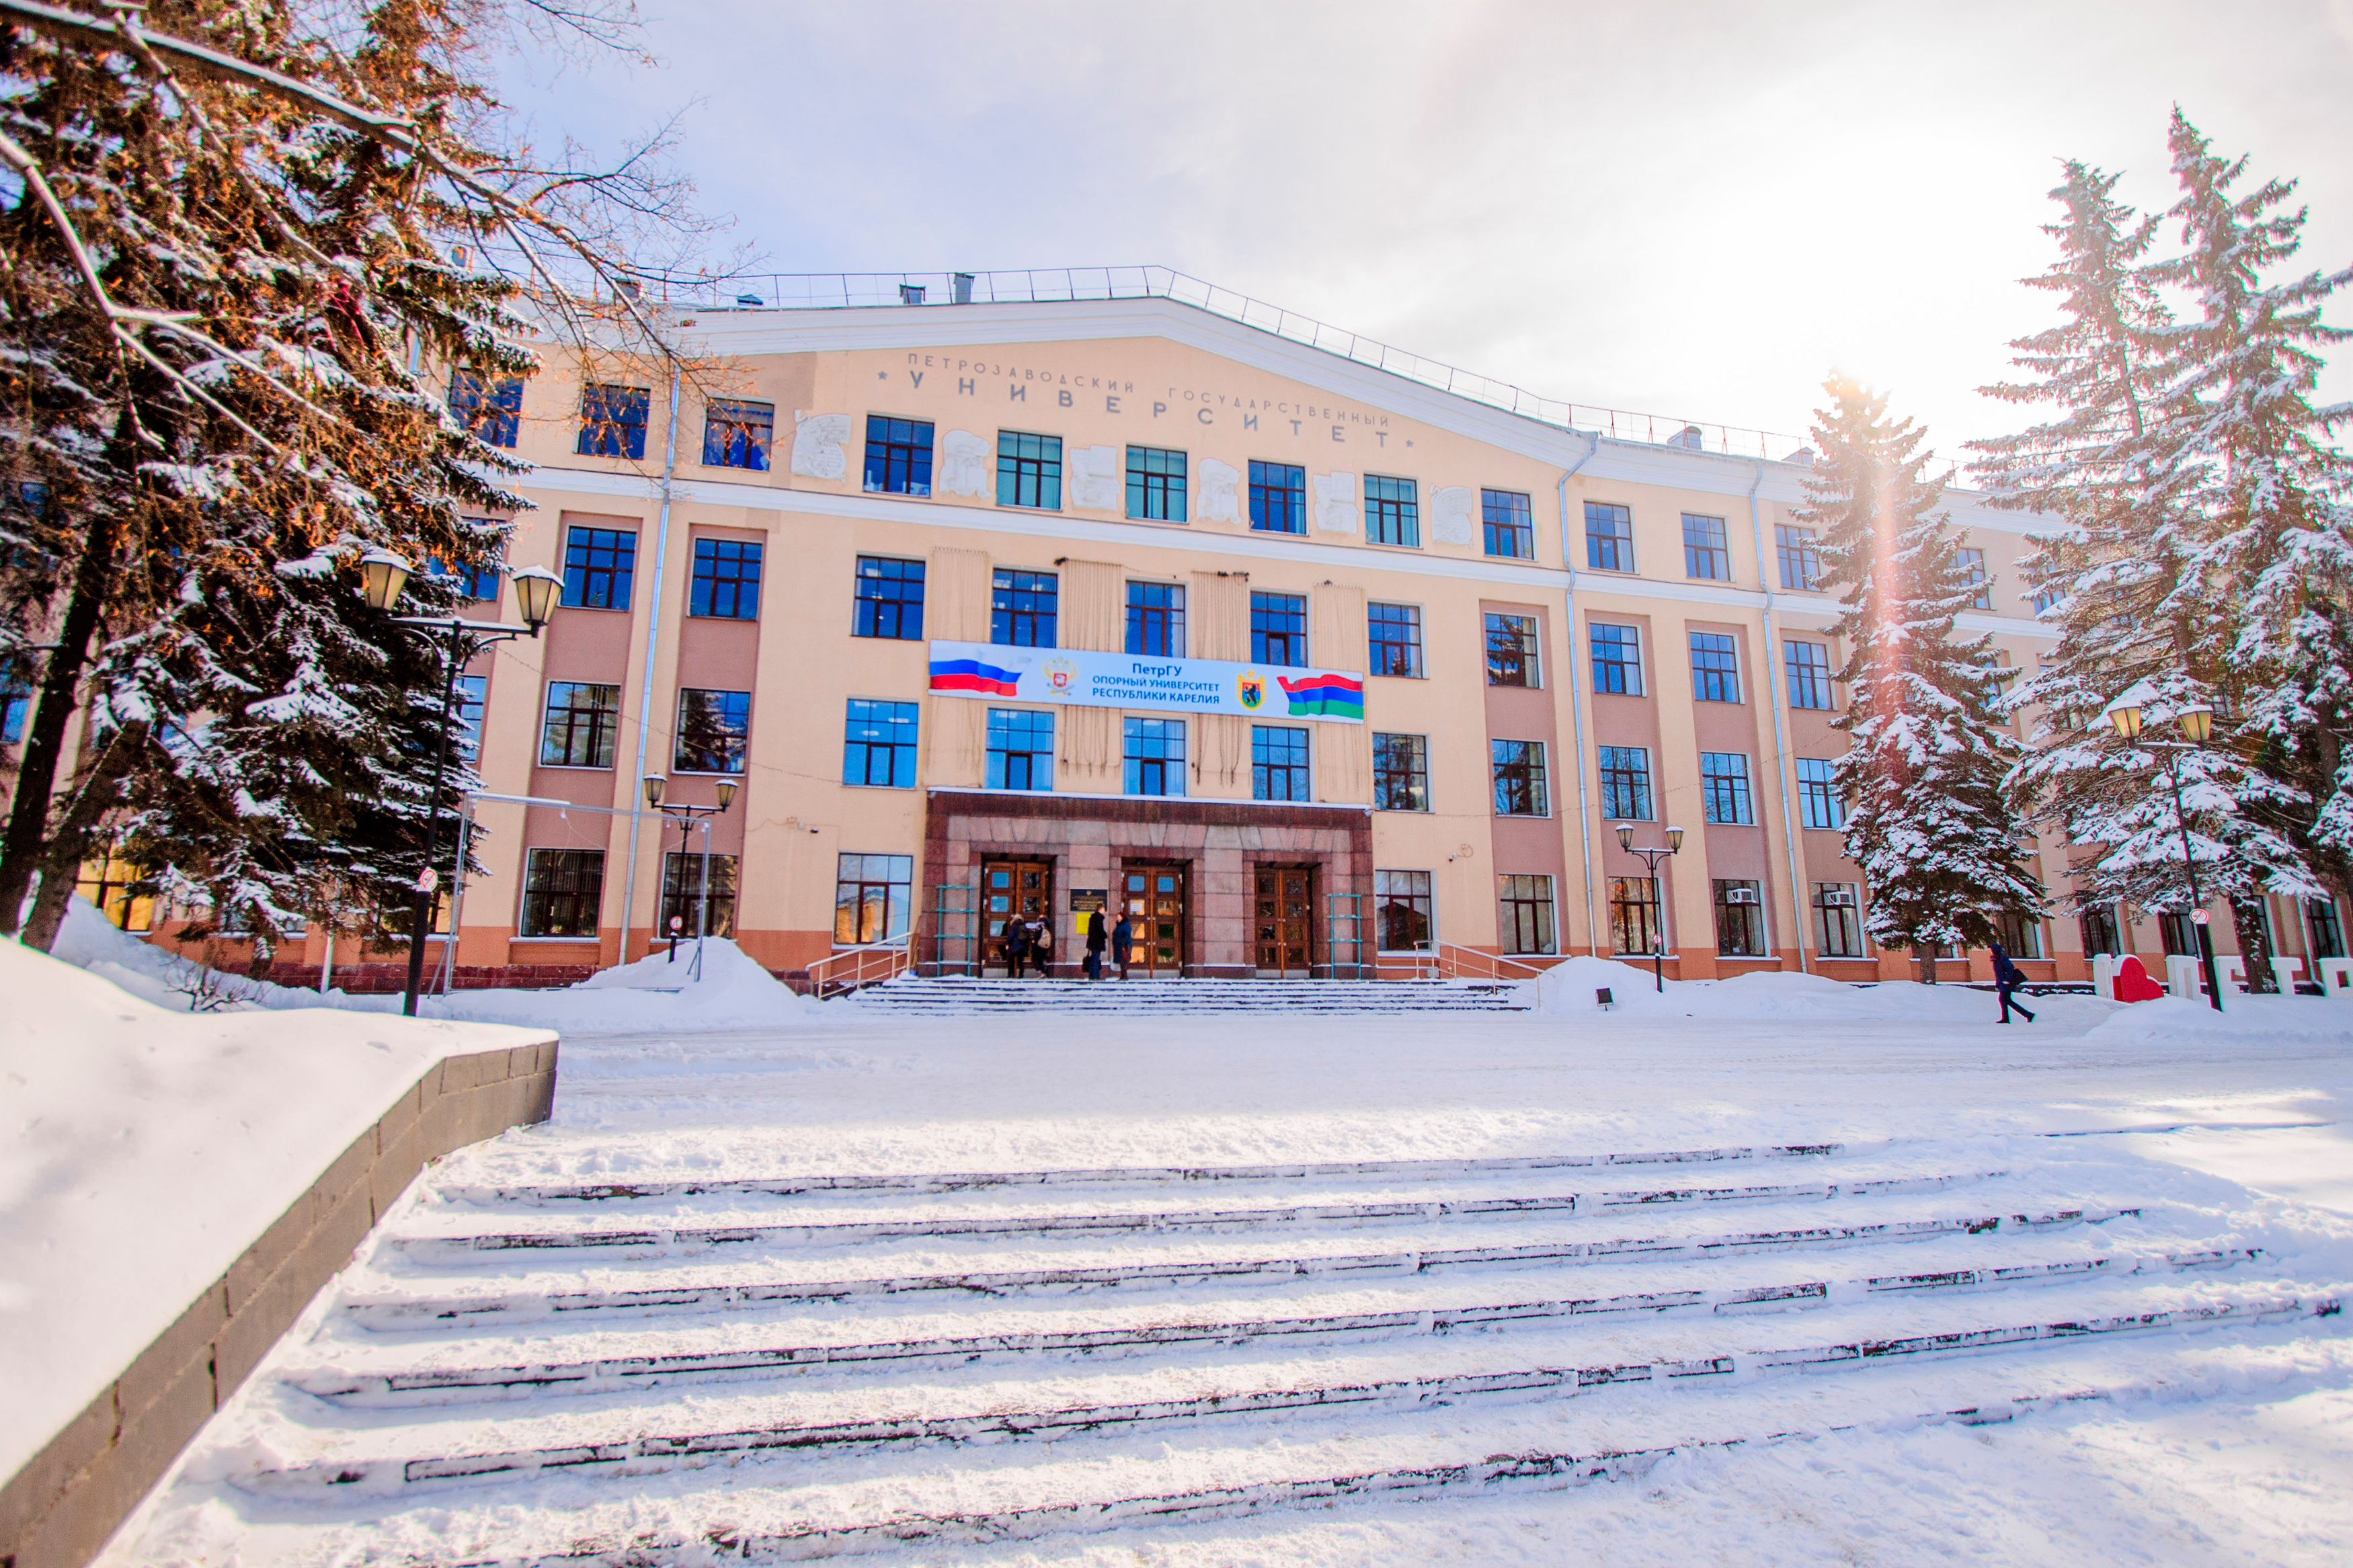
\includegraphics[height=4.5cm, width=7cm, keepaspectratio=true, clip=true, trim = {0 6cm 0 6cm}]{images/petrsu.jpg}
        \end{center}
        \end{block}
    \end{column}
    }
    
  \end{columns}
\end{frame}